\documentclass[12pt]{article}

\usepackage{enumitem}
\usepackage[right=20mm, left=20mm]{geometry}
\usepackage{type1cm}
\usepackage{amssymb}
\usepackage[fleqn]{amsmath}
\usepackage{tikz}
\usepackage{multicol}
\usepackage{makecell}
\setlength{\columnsep}{1pt}
\usepackage{pgfplots}
\usepackage{float}
\usepackage{caption}
\usepackage{subcaption}
% \usepackage{subfig}
\usepackage{graphicx}

\usepackage{indentfirst}
\usepackage{lastpage}  
\usepackage{fancyhdr}
\pagestyle{fancy}

\usepackage[unicode=true,pdfusetitle,
 bookmarks=true,bookmarksnumbered=false,bookmarksopen=false,
 breaklinks=false,pdfborder={0 0 1},backref=false,colorlinks=false]
 {hyperref}

\makeatletter
\newenvironment{myalign*}{\ifvmode\else\hfil\null\linebreak\fi
  \hspace*{-\leftmargin}\minipage\textwidth
  \setlength{\abovedisplayskip}{0pt}%
  \setlength{\abovedisplayshortskip}{\abovedisplayskip}%
  \start@align\@ne\st@rredtrue\m@ne}%
{\endalign\endminipage\linebreak}

% Paper size
\topmargin -10mm
\textwidth 170mm
% \oddsidemargin -5mm
% \evensidemargin -5mm
\textheight 220mm

% Font setting
\usepackage{xeCJK}
% \setCJKmainfont{Noto Sans TC}
\setCJKmainfont{kaiu.ttf}


\renewcommand{\footnotesize}{\normalsize} 
\renewcommand{\headrulewidth}{0pt}
\renewcommand{\footrulewidth}{0pt}

\lhead{}
\chead{2023年全國大專校院智慧創新暨跨域整合創作競賽系統需求書}
\rhead{}

\lfoot{}
\cfoot{}
\rfoot{ 共 \pageref{LastPage} 頁 第  \thepage   頁} 

\makeatletter
\begin{document}
% \fontsize{14pt}{18pt}\selectfont
% \author{}
\date{}
\usetikzlibrary{automata, positioning, arrows}
% \maketitle
\tikzset{every state, accepting/.style={double distance=2pt}}
\captionsetup[figure]{labelfont={bf},name={圖},labelsep=period}

\noindent
\textbf{參賽隊名:} 普羅程式 \\
\textbf{作品名稱:} 威力導師 PowerTeacher \\

\begin{enumerate}
  \setlength{\parindent}{2em}
  \item 系統名稱
  \par 威力導師
  \item 系統目的與範圍
  \par 在台灣,資訊科技領域備受關注,且程式設計已成為學校必修課程。儘管每年有數百萬學生修習程式課程,但基層教育仍面臨著許多問題:以往的教學方式需頻繁切換畫面給學生練習、課堂上教師無法即時得知學生狀況。所以我們建立一個名為PowerTeacher的網頁應用,專注於教師導向的程式教學工具,整合直播、實作、測驗、互動與AI輔助,讓所有人都能進行優質的程式教學。

  \newpage % 換頁
  \item 系統非功能需求
  \begin{table}[htb]
    \centering
    \begin{tabular}{|c|p{8cm}|}
        \hline
        \textbf{代號} & \textbf{非功能需求} \\
        \hline
        NFR-001 & 使用者介面與人為因素 \\ 
        & $\bullet$ 使用者:程式設計課程的老師、學生 \\
        & $\bullet$ 使用者的介面設計:簡單並且易上手、高度的功能整合、即時獲得使用者的反饋與資訊。 \\
        & $\bullet$ 使用者的引導與教學:直觀的 UI 設計並且將編輯功能視覺化。\\
        \hline
        NFR-002 & 設備需求 \\
        & $\bullet$ 使用者的使用設備:使用設備以電腦為主、手持設備為輔,並針對電腦使用最佳化。\\
        & $\bullet$ 使用者的設備限制:所有能瀏覽網頁的設備皆可使用。\\
        \hline
        NFR-003 & 效能需求 \\
        & $\bullet$ 反應時間:同一課程能讓 100 人同時使用,並在 0.1 秒內回應使用者,以保障使用者的上課體驗。\\
        & $\bullet$ 容量限制:限制每位教師在單一章節中,只能上傳 20MB 以下的投影片。\\
        & $\bullet$ 課堂限制:每位教師的課程需要經過管理員審核後才能開課,並且每位教師以開設 5 門課為限。\\
        & $\bullet$ 課堂人數:同一課程最多只能有 100 位學生。\\
        \hline
        NFR-004 & 錯誤處理 \\
        & $\bullet$ 系統遇到不正常的負載:針對大量請求的用戶限制封包的流量。\\
        & $\bullet$ 系統遇到高負載:使用排隊來限制同時登入人數。\\
        \hline
        % 在這裡添加其他非功能需求...
        % NFR-002, NFR-003, ...
        % 將其他需求按相同的格式添加到表格中
    \end{tabular}
    \caption{非功能需求列表}
  \end{table}


  \item 系統功能需求
  
  \begin{table}[htb]
    \centering
    \begin{tabular}{|c|c|}
      \hline
      用例名稱 & \\ \hline
      參與者 & \\ \hline
      前置條件 & \\ \hline
      事件流程 & \\ \hline
      例外事件流程 & \\ \hline
      後置條件 & \\ \hline
    \end{tabular}    
  \end{table}

  % \begin{figure}[htb]
  %   \centering
  %   \begin{subfigure}{0.45\linewidth}
  %     \centering
  %     \href{https://raw.githubusercontent.com/programingtw/proglearn-plan/main/img/arc1.jpg}{
  %       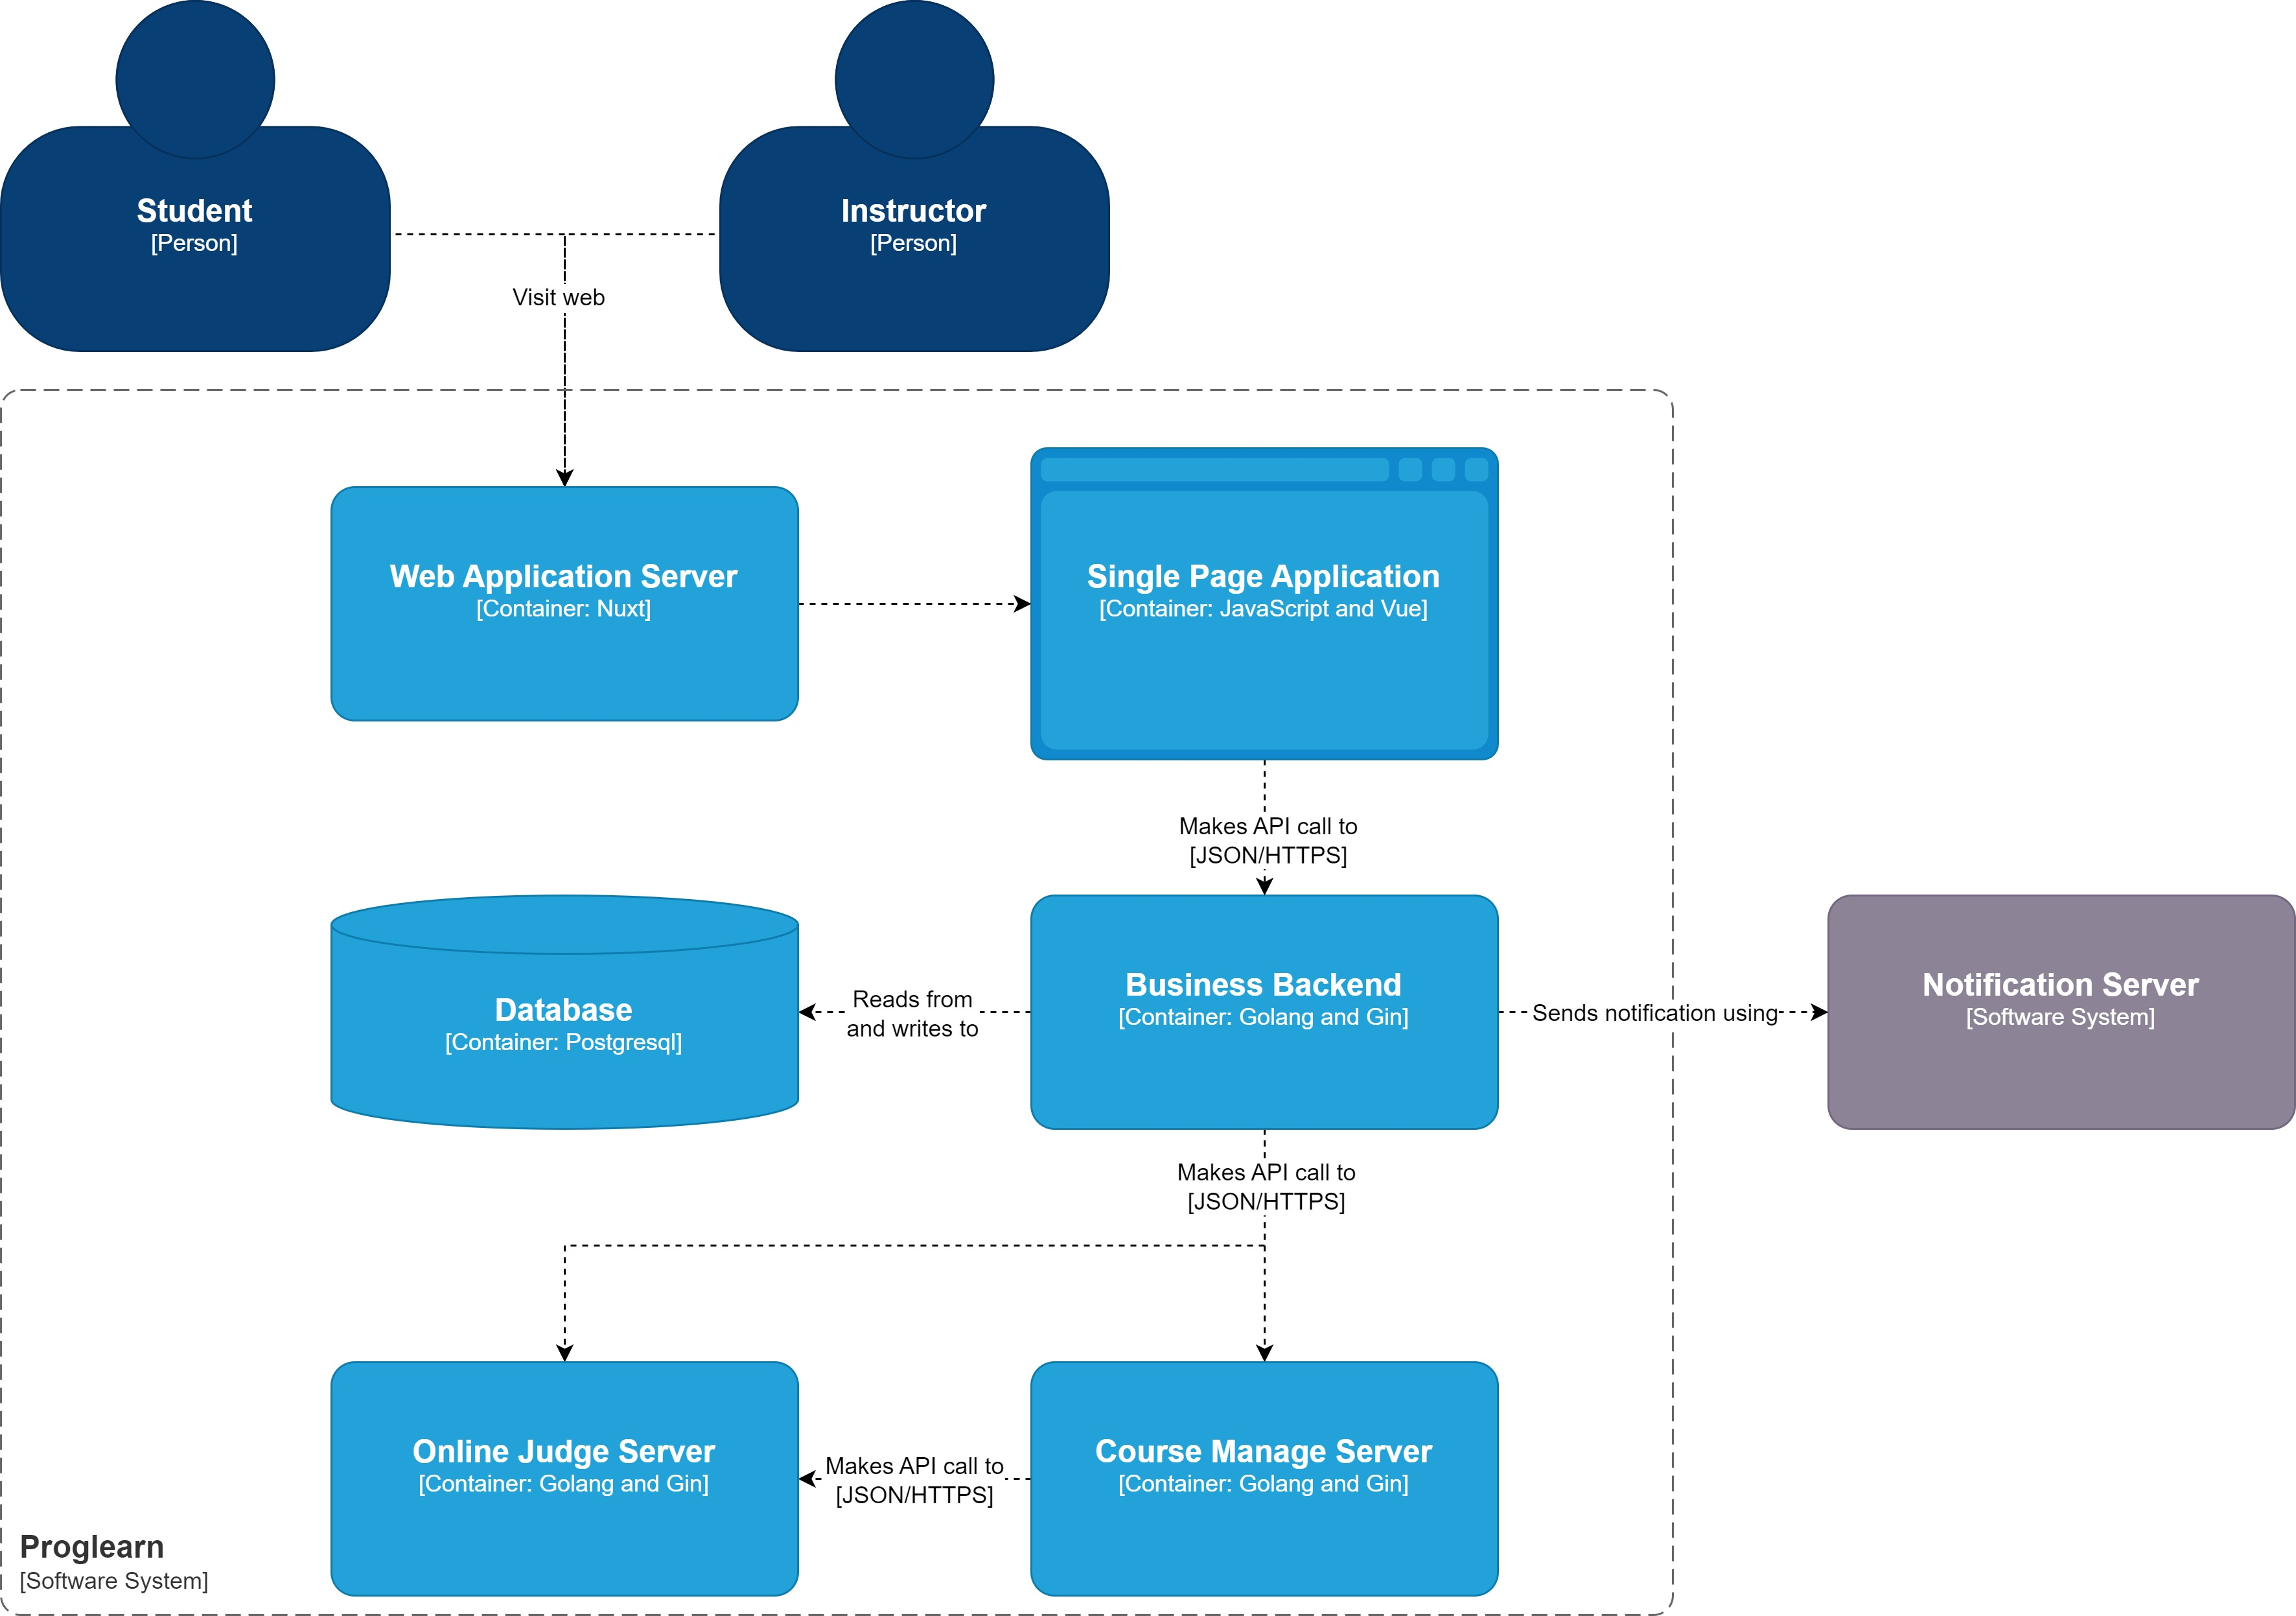
\includegraphics[width=0.65\textwidth]{./img/arc1.jpg}
  %     }
  %     \caption{CAPTION}
  %     \label{arc1}            
  %   \end{subfigure}
  % \end{figure}
\end{enumerate}
\end{document}